
%% ANÁLISE EXPLORATORIA

%%% Gráfico da série

No painel (a) da Figura \ref{fig:cap2_asg_o3_pinheiros}, apresentamos o gráfico da série horária de ozônio medida na estação de monitoramento de Pinheiros, São Paulo, no período de 2008 a 2013 \citep{Salvo2017}. Podemos observar a existência de um pequeno período sem informação no segundo semestre de 2009 e a tendência da concentração de ozônio ser maior nos últimos meses de cada ano. 

Quando as séries têm muitas observações, seus gráficos ficam muito densos, o que pode tornar difícil a identificação de padrões. Uma solução para isso é visualizar o gráfico da série suavizada. No painel (b) da Figura \ref{fig:cap2_asg_o3_pinheiros}, apresentamos a concentração de ozônio acrescida da sua série suavizada por \textit{splines cúbicos} (ver Seção \ref{sec:gam-splines}), o que torna o padrão sazonal mais evidente. Uma outra alternativa é diminuir a frequência da série. Nesse sentido, apresentamos no painel (c) a série diária medida às 14h (horário de pico do ozônio). Note que a série diária carrega o mesmo padrão sazonal da série horária. 

Além de analisar as características de uma série isoladamente, podemos plotar duas ou mais séries conjuntamente para investigar a associação entre elas. No painel (d) da Figura \ref{fig:cap2_asg_o3_pinheiros}, apresentamos o gráfico da temperatura média para a cidade de São Paulo medida nos mesmos instantes que o ozônio. Observamos que os picos de temperatura também ocorrem entre novembro e fevereiro, sugerindo uma associação positiva entre temperatura e concentração de ozônio.


\begin{figure}[h!]
	\centering
	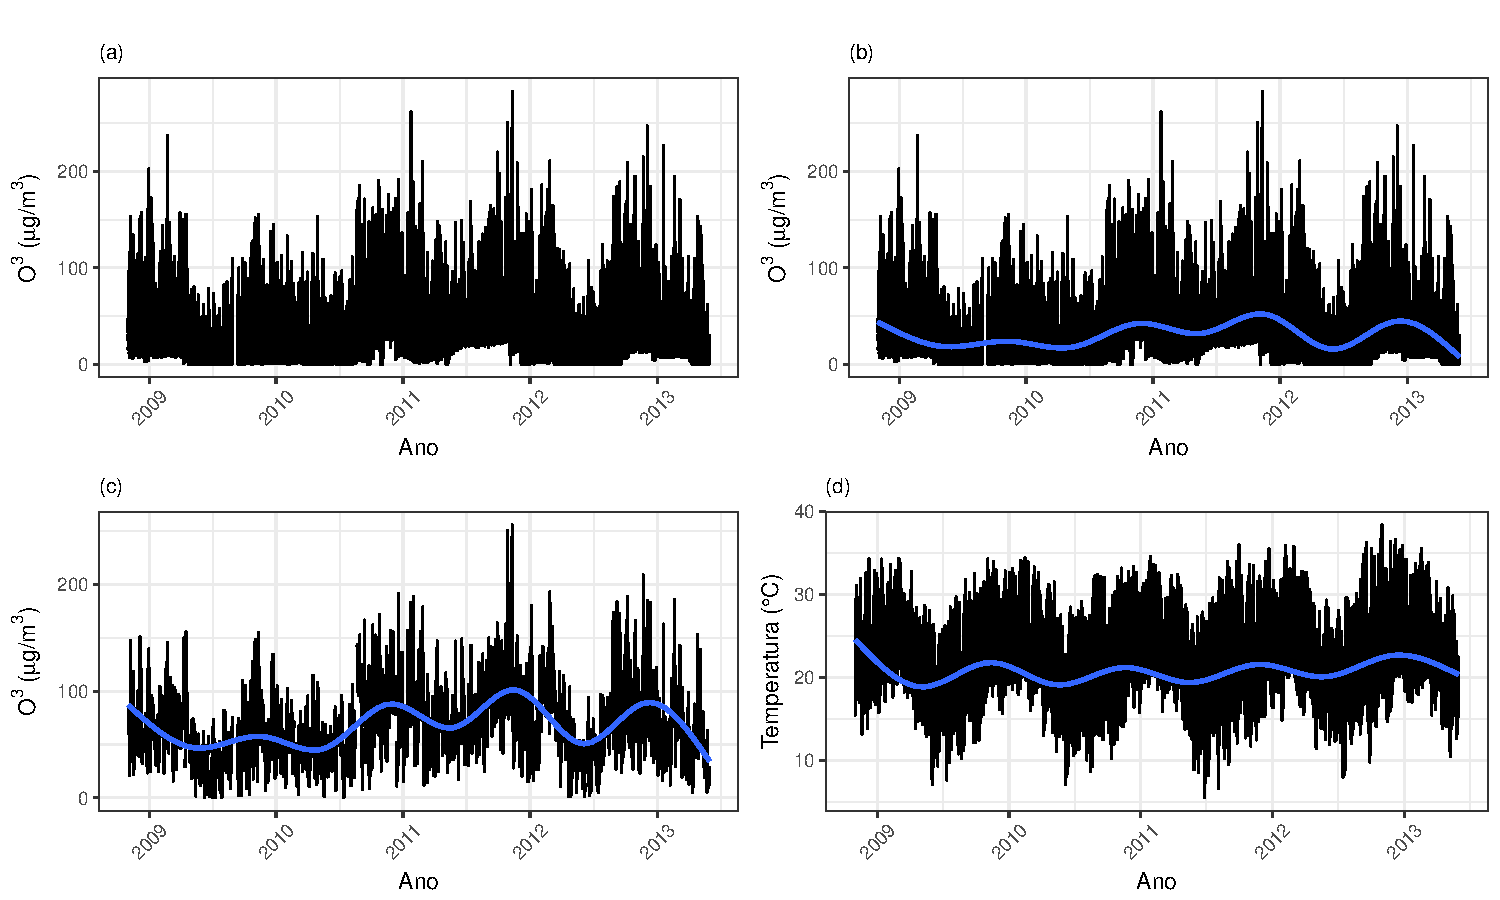
\includegraphics[width=\linewidth]{../analise-poluicao/img_tese/cap2_asg_o3_pinheiros.pdf}
	\caption{Exemplos de gráficos de séries. Temperatura e concentração de ozônio para a cidade de São Paulo de outubro de 2009 a junho de 2013. Ozônio medido na estação de monitoramento de Pinheiros. Dados disponibilizados por \cite{Salvo2017}. (a) Série horária da concentração de ozônio. (b) Série horária da concentração de ozônio acrescida da série suavizada. (c) Série diária da concentração do ozônio medida às 14h. (d) Série horária da temperatura.}
	\label{fig:cap2_asg_o3_pinheiros}
\end{figure}

Nesse estudo \citep{Salvo2014}, um dos objetivos dos autores era associar a proporção de carros a gasolina no município de São Paulo com a concentração de ozônio. Apresentamos a série da proporção de carros a gasolina no período estudado na Figura \ref{fig:cap2_asg_share_gas}, acrescida da sua suavização, agora linear. Observe que a proporção tende a aumentar ao longo do tempo, indicando uma tendência positiva, isto é, sua média aumenta com o tempo.

\begin{figure}[h!]
	\centering
	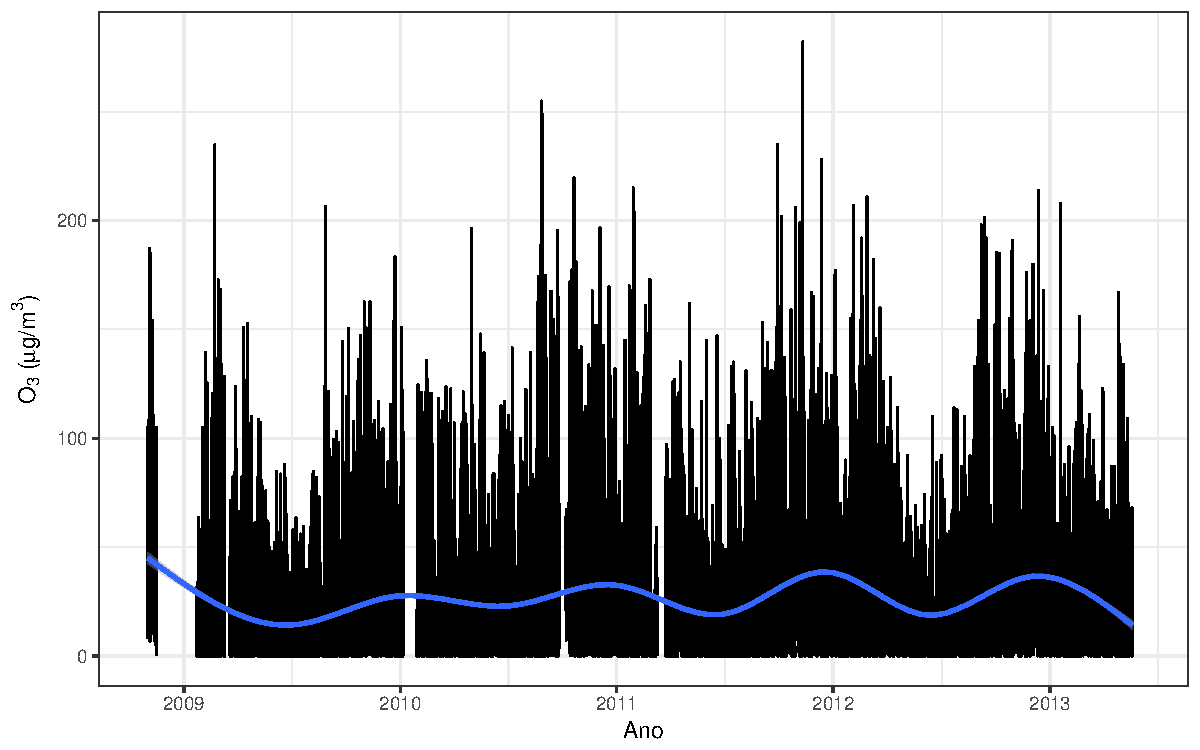
\includegraphics[width=\linewidth]{../analise-poluicao/img_tese/cap2_asg_share_gas.pdf}
	\caption{Série da proporção de carros a gasolina na cidade de São Paulo no período de outubro de 2009 a junho de 2013. Dados disponibilizados por \cite{Salvo2017}.}
	\label{fig:cap2_asg_share_gas}
\end{figure}

Tendência implica em não-estacionariedade, o que viola uma suposição crítica para a inferência em séries temporais. A estacionariedade permite a extrapolação das conclusões retiradas da amostra para um contexto mais geral e, por isso, as principais metodologias para séries temporais fazem essa suposição. Na próxima seção, discutiremos esses conceitos com mais detalhes. 

%%% Estacionariedade

Para introduzirmos formalmente o conceito de estacionariedade, precisamos definir a \textit{função de autocovariância}. Considere uma série $Y_t$. Denotamos sua média\footnote{Quando $\mu_t$ não é constante ao longo do tempo, isto é, depende do instante $t$, dizemos que a série apresenta tendência. Se essa tendência assume um padrão cíclico, em um intervalo fixo de tempo, dizemos que a série é sazonal.} e sua variância, respectivamente, por $\mu_t = E(Y_t)$ e $\sigma^2_t = VAR(Y_t)$. Se a variância da série for finita para todo $t \geq 1$, definimos a função de autocovariância de $Y_t$ como

\begin{displaymath}
\gamma(t,s) = E\left[(Y_t - \mu_t)(Y_s - \mu_s)\right].
\end{displaymath}

A função de autocovariância pode ser estimada pela função de autocovariância amostral, definida por

\begin{equation}
\hat{\gamma}(h) = \frac{1}{n}\sum_{t=1}^{n-h}(y_{t+h} - \bar{y})(y_t - \bar{y}),
\label{def:sample-autocov}
\end{equation}
sendo $y_t$ o valor observado no instante $t$ e $\bar{y} = \frac{1}{n}\sum_{t=1}^{n}y_t$ a média amostral.

Séries heteroscedásticas \footnote{Séries cuja variância não é constante ao longo do tempo.} podem ser transformadas para se alcançar a estabilização da variância. As principais transformações utilizadas com esse objetivo envolvem funções linearizadoras, como a $\log{Y_t}$ ou $\sqrt{Y_t}$. Ao custo de interpretabilidade, essas transformações comprimem a escala da variável, tornando seus valores mais próximos e diminuindo a oscilação da variância. Essa estratégia também é bastante utilizada em modelos de regressão que supõem variáveis homoscedásticas. Falaremos com mais detalhes sobre esse tema no contexto de regressão na Seção \ref{sec:heteroscedasticidade}.

%%%

Dessa maneira, denotamos (\ref{y-equal-X-Z-e}) como

\begin{displaymath}
Y_t = f(\mathbf{X_t}, \mathbf{Z_t}) + \epsilon_t,
\end{displaymath}
sendo 

A análise de séries temporais reúne técnicas desenvolvidas para estudar a correlação temporal existente em observações ou variáveis amostradas ao longo do tempo. De um modo geral, as metodologias podem ser divididas entre abordagens no domínio temporal e no domínio das frequências. O foco da abordagem temporal é estudar a \textit{autocorrelação} entre as observações, isto é, como e quanto cada observação está associada aos valores medidos em instantes anteriores. Já a abordagem no domínio das frequência mira a periodicidade da série, isto é, a investigação dos padrões da série ao longo do tempo.

A variável resposta será denotada aqui por $Y_t$, sendo $t = 1, 2, 3, \dots$ a ordem em que as observações foram amostradas. Quando existirem, denotaremos as $p$ variáveis explicativas por $X_{1t}, \dots, X_{pt}$. Quando não houver chance de confusão, omitiremos o índice $t$ da notação.


%%%%%
%% Modelos espaço estado

\section{Modelos espaço-estado}

Estudos de poluição atmosférica envolvem dados cuja coleta é naturalmente suscetível à omissão. A medição de poluentes e de variáveis meteorológicas, por exemplo, envolve equipamentos que estão sujeitos a imprecisões, falhas e precisam ser constantemente regulados. Esses dados geralmente são sustentados pela administração pública, cuja redução de verbas pode descontinuar ou reduzir os planos de coleta.

Às vezes, o próprio delineamento do estudo gera dados faltantes. Na análise feita por \cite{Salvo2014}, os autores descartaram da amostra os meses frios (julho à setembro), devido à menor formação de ozônio nesse período. Por causa da influência do tráfego no estudo, os feriados e fins de semanas também não foram considerados. \hl{Essas exclusões geraram uma série cheia de buracos, o que dificulta a aplicação de certas técnicas.}

De uma forma geral, os dados faltantes diminuem a representatividade da amostra e podem gerar distorções na inferência sobre a população. Quando não é possível evitar a omissão, precisamos utilizar modelos robustos a dados faltantes ou técnicas que amenizam o seu efeito.

Uma técnica muito utilizada é a imputação. [...]

No contexto de séries temporais, os modelos espaço-estado são uma boa alternativa para modelar séries com dados faltantes. [...]

Neste capítulo, discutiremos as principais estratégias para a análise de dados de poluição atmosférica na presença de grandes períodos sem observação.

%%%%%%%%%%%%%%%%%%

Os modelos espaço-estado (ou modelos lineares dinâmicos) foram introduzidos por \cite{Kalman1960} e \cite{Kalman1961} como uma generalização de diversos casos especiais de interesse. 

Os modelos espaço-estado são caracterizados por duas suposições principais. A primeira afirma que a verdadeira variável sob estudo, $U_t$, é um fenômeno não-observável. Neste caso, o que realmente observamos é uma transformação linear desse fenômeno, $A_tU_t$, acrescida de um ruído, $v_t$. A segunda suposição diz respeito sobre o processo de geração de $U_t$. Mais precisamente, na sua forma mais básica, temos que $U_t$ é gerado por um processo autoregressivo de primeira ordem.

Dadas essas duas suposições, podemos escrever o modelo de espaço-estado da seguinte maneira

\begin{displaymath}
Y_t = a_tU_t + v_t
\end{displaymath}
\begin{equation}
U_t = \phi U_{t-1} + w_t,
\label{mod:espaco-estado}
\end{equation}
sendo $a_t$ e $\phi$ parâmetros do modelo e $w_t \sim N(0, \sigma_w)$. A primeira equação em (\ref{mod:espaco-estado}) é chamada de \textit{equação de estado}, enquanto a segunda é chamada de \textit{equação de observação}.


%% Normalidade

%\subsection{Normalidade}
%
%A distribuição Normal assume que a variável aleatória está definida na reta real, isto é, pode assumir valores positivos e negativos, e é simétrica em relação a sua média. Intuitivamente, não há motivos para acreditar que essa distribuição se ajustaria bem a dados naturalmente positivos e assimétricos, como a concentração de poluentes e número de casos de uma doença ou mortalidade. Mesmo assim, pela facilidade de implementação e interpretação, o modelo normal é muitas vezes utilizado como uma primeira tentativa na estratégia de análise, de tal forma que, se os dados não se afastarem muito desta distribuição, pequenos vieses podem ser negligenciado em favor de um modelo mais simples.
%
%Como mencionado anteriormente, o método de mínimos quadrados não supõe normalidade no processo de estimação. Apesar de essa suposição ser feita na construção de intervalos de confiança e testes de hipóteses para os parâmetros, para amostras grandes\footnote{Comum em estudos de poluição do ar.}, a teoria assintótica garante estimadores com distribuição aproximadamente normal \REF. No entanto, como a velocidade dessa convergência depende da natureza (desconhecida) da variável sob estudo, não temos como quantificar o que é uma ``amostra grande'', o que justifica a importância de se avaliar a qualidade do ajuste em relação à suposição de normalidade. 
%
%Uma primeira ideia para checar essa suposição seria construir o histograma da variável resposta e avaliar se ele se aproxima de uma distribuição normal. Contudo, a suposição de normalidade se refere à variável $Y|\mathbf{X}, \mathbf{Z}$ e não a $Y$ simplesmente. Seria necessário construir histogramas para cada combinação de valores de $\mathbf{X}$ e $\mathbf{Z}$, o que é quase sempre impossível.
%
%Gráficos Q-Q (quantil-quantil) e envelopes \REF são técnicas muito úteis para investigar possíveis desvios da suposição de normalidade. Eles se baseiam nos resíduos studentizados \REF e avaliam o quanto a distribuição empírica desses resíduos se afasta da distribuição teórica. \Ex
%
%%Atkinson, A. C. (1985). Plots, Transformations and Regressions. Oxford Statistical Science Series, Oxford.
%
%A transformação da variável $Y$ pode ser uma alternativa para casos em que a suposição de normalidade não é válida. As transformações $\log Y$ e $\sqrt{Y}$ são as mais utilizadas. Na Seção \ref{cap:glm}, veremos como generalizar o modelo linear para outras distribuições.


%%% VALIDAÇÃO CRUZADA

Muitas vezes, quando a classe de modelos escolhida exige a escolha de hiperparâmetros, como o grau de suavização de um modelo aditivo generalizado (Seção \ref{sec:gam}) ou o $\lambda$ do LASSO (Seção \ref{sec:lasso}), é comum separarmos a amostra em três partes: uma amostra de treino, uma amostra de validação e uma amostra de teste. Nesse caso, os modelos são treinados com a amostra de treino e, para diversos valores do hiperparâmetro, calculamos o erro de teste na amostra de validação. Escolhemos então o hiperparâmetro que leva ao menor erro de teste e utilizamos a amostra de teste para calcular o erro de teste do modelo final. Geralmente utiliza-se LOOOCV ou \textit{k-fold} para a validação e uma amostra separada para o teste. Essa estratégia é utilizada para garantir que o erro de teste não seja calculado em observações utilizadas no ajuste do modelo e reflita o erro que obteríamos ao aplicá-lo no mundo real.


%% LIME RF SALVO 2017

Uma maneira alternativa de interpretar os dados é utilizar o LIME, discutido na Seção \ref{sec:lime}. Para cada observação na base, nós aplicamos o LIME para explicar os preditores que mais influenciaram em sua própria predição. A Figura \ref{fig:cap-comb-lime-pinheiros} apresenta a proporção estimada de carros a gasolina contra o coeficiente estimado para esse preditor no modelo simples (regressão \textit{ridge}). Podemos observar que, para valores da proporção estimada de carros a gasolina menor que 0.48, há modelos que consideram esse preditor tanto negativamente quanto positivamente associado ao ozônio. A partir de 0.48, os coeficientes do modelo simples são predominantemente negativos. Esse resultado reforça dois indícios encontrados nas análises apresentadas até aqui. Primeiro, não é clara a relação entre a proporção estimada de carros a gasolina e a concentração de ozônio quando o valor deste preditor é menor que 50\% (aproximadamente). Segundo, quando a proporção estimada de carros a gasolina está aproximadamente 50\% e 60\%, todos os modelos sugeriram uma associação negativa com a concentração de ozônio.

\begin{figure}[h!]
	\centering
	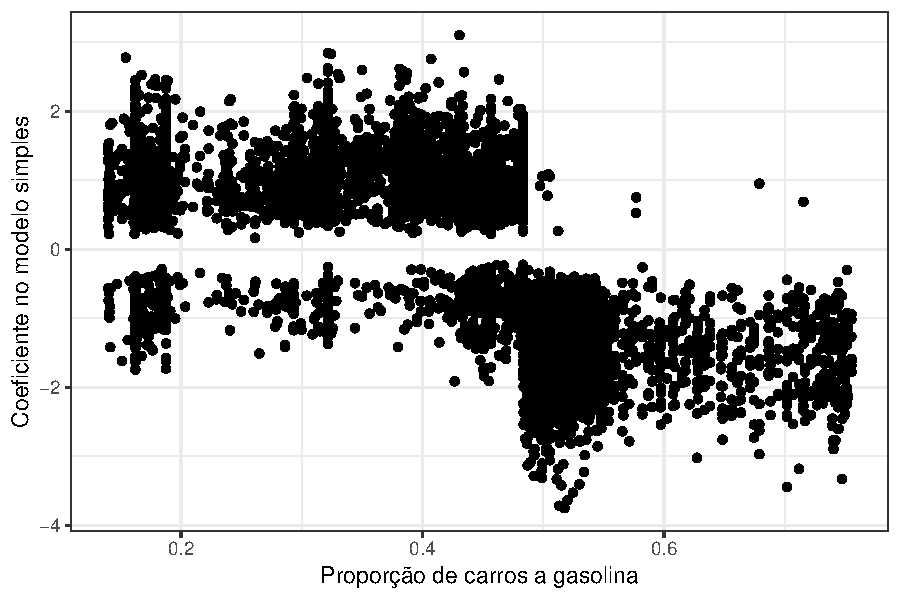
\includegraphics[width=0.7\linewidth]{figuras/cap-comb-rf-explanation.pdf}
	\caption{Proporção estimada de carros a gasolina contra o coeficiente estimado para esse preditor no modelo simples (regressão \textit{ridge}).}
	\label{fig:cap-comb-lime-pinheiros}
\end{figure}

Como a suposição de que a proporção de carros a gasolina não está associada diretamente a nenhum outro preditor, podemos predizer o ozônio substituindo o verdadeiro valor da proporção por um valor hipotético, que simule um cenário com poucos carros a gasolina rodando na cidade e outro com muito carros a gasolina. Na Figura \ref{fig:cap-comb-random-forest-cenarios}, apresentamos as curvas suavizadas do ozônio predito para esses dois cenários, além do cenário de fato observado. Os valores fixados para a proporção de carro a gasolina foram: 20\% para representar o cenário com poucos carros a gasolina e 70\% para o cenário com muitos carros. Esses valores foram escolhidos com base na distribuição da variável original. Observamos pelo gráfico que, os cenários observado e com baixa proporção são bem parecidos, enquanto o cenário com alta proporção apresenta menores concentrações em algumas estações.

\begin{figure}[h!]
	\centering
	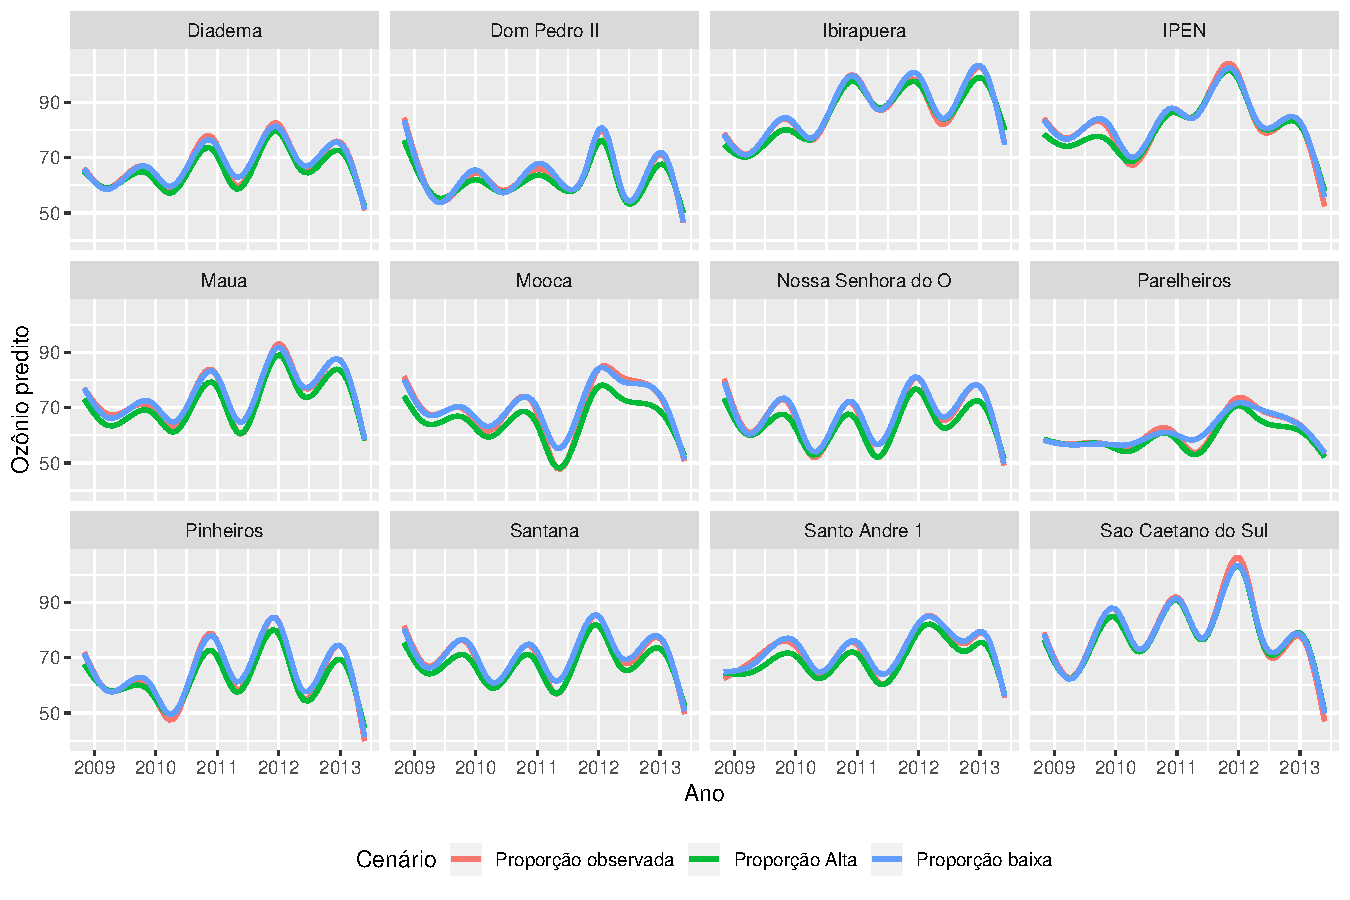
\includegraphics[width=0.7\linewidth]{figuras/cap-comb-random-forest-cenarios.pdf}
	\caption{Curvas suavizadas do ozônio predito para os cenários observado, com alta proporção de carros a gasolina (70\% durante todo o período) e baixa proporção de carros a gasolina (20\% durante todo o período).}
	\label{fig:cap-comb-random-forest-cenarios}
\end{figure}